\documentclass[letterpaper,12pt]{article}
\usepackage{graphicx}
\graphicspath{{./images/}}
\usepackage{amssymb}
\usepackage{amsmath}
\usepackage{amstext}
\usepackage{subcaption}
%\usepackage{subfigure}
\usepackage{url}
\usepackage{color}
\usepackage{hyperref} \hypersetup{pdfborder={0 0 0}}
\usepackage{circuitikz}
\usepackage[framemethod=tikz]{mdframed}
\usetikzlibrary{shapes.geometric}
\usetikzlibrary{fit}
\usepackage{anyfontsize}
%% Tikz settings for flowcharts
\definecolor{blockcolor}{RGB}{255,252,204}
\tikzstyle{block} = [draw, fill=blockcolor, rectangle,
    minimum height=3em, minimum width=6em,align=center]
\tikzstyle{sum} = [draw, fill=white, circle, node distance=1cm]
\tikzstyle{input} = [coordinate]
\tikzstyle{output} = [coordinate]
\tikzstyle{outputMiddle} = [coordinate]
\tikzstyle{pinstyle} = [pin edge={to-,thin,black}]
%%%
\newmdenv[
linewidth=1pt,
innerrightmargin=80pt,
singleextra={
  \path let \p1=(P), \p2=(O) in
  node[xshift=-40pt] at (P|-0,0.5*\y1+0.5*\y2)
    {\fontsize{100}{120}\selectfont ?};
}
]{Qbox}

\newcommand\questionbox[1]{%
  \begin{Qbox}#1\end{Qbox}}
%%%
%% Tikz settings for flowcharts
\definecolor{blockcolor}{RGB}{255,252,204}
\tikzstyle{block} = [draw, fill=blockcolor, rectangle,
    minimum height=3em, minimum width=6em,align=center]
\tikzstyle{sum} = [draw, fill=white, circle, node distance=1cm]
\tikzstyle{input} = [coordinate]
\tikzstyle{output} = [coordinate]
\tikzstyle{outputMiddle} = [coordinate]
\tikzstyle{pinstyle} = [pin edge={to-,thin,black}]
\addtolength{\oddsidemargin}{-.875in}
\addtolength{\evensidemargin}{-.875in}
\addtolength{\textwidth}{1.75in} \addtolength{\topmargin}{-.875in}
\addtolength{\textheight}{1.75in} \special{papersize=\the\paperwidth,\the\paperheight}

\begin{document}

\begin{table}[h]
\begin{tabular}{cc}
  
\includegraphics[width=2in,keepaspectratio=true]{images/logo.eps} &
  \begin{tabular}{c}
    \vspace*{0.5cm}{\large ECE4305: Software-Defined Radio Systems and Analysis} \\
    \vspace*{0.1cm}{\large Laboratory 2: Carrier Synchronization} \\
  \end{tabular}\\
  \hline
\end{tabular}
\end{table}

\section*{Objective} This laboratory will introduce the concept of carrier frequency offset between transmitting and receiving nodes. Specifically, a simplified error model will be discussed along with two recovery methods which can operate jointly or independently, based on their implementation. Carrier recovery complements timing
recovery, which was implemented in Lab 1, and is necessary for maintaining wireless links between radios with independent oscillators.
\tableofcontents

\newpage

\section{Theoretical Preparation}
The fundamental concepts of digital communication systems and related theoretical background material covered in this section will serve as a basis for the implementation and design of prototype systems throughout the rest of this course.

\subsection{System and Error Models}\label{sec:models}
Throughout this Lab we will assume that timing mismatches between the transmitting and
receiving radios have already been corrected. However, this is not a requirement in all cases, specifically in
the initial implementation provided here, but will become a necessary condition for optimal performance
of the final implementation provided. For the sake of simplicity we will also ignore timing effects in
our simulations except when discussing PlutoSDR itself, since obviously timing correction cannot be
overlooked in that case. With regards to our full receiver diagram outline in Figure~\ref{rbd}, we are now
considering the Carrier Recovery and CFO blocks.\par
%
\begin{figure}[!htp]
 \centering
 \begin{tikzpicture}[auto, node distance=2cm,>=latex']
  \tikzstyle{block} = [draw, fill=blockcolor, rectangle,
      minimum height=3em, text width={width("Equalization")+0pt},align=center]
  \tikzstyle{blockhl} = [draw, dashed, , fill=blue, rectangle,
  minimum height=3em, text width={width("Equalization")+0pt},align=center]
    % Blocks and positions
    \node [input, name=input] {};
    \node [blockhl, right of=input, node distance=2.2cm] (cfo) {CFC};
    \node [block, right of=cfo, node distance=3cm] (mf) {Matched Filter};
    \node [block, right of=mf, node distance=3cm] (tr) {Timing Recovery};
    \node [blockhl, right of=tr, node distance=3cm] (cf) {Carrier Recovery};
    \node [block, right of=cf, node distance=3cm] (fs) {Frame Sync};
    \node [block, right of=fs, node distance=3cm] (eq) {Equalization};
    \node [output, right of=eq, node distance=2.2cm] (output) {};
    % Lines
    \draw [draw,->] (input) -- node {} (cfo);
    \draw [->] (cfo) -- node {} (mf);
    \draw [->] (mf) -- node {} (tr);
    \draw [->] (tr) -- node {} (cf);
    \draw [->] (cf) -- node {} (fs);
    \draw [->] (fs) -- node {} (eq);
    \draw [->] (eq) -- node {} (output);
    %\draw [dashed] (a) -- (b);
\end{tikzpicture}
  \caption{Receiver Block Diagram.}
  \label{rbd}
\end{figure}
%
The receiving and transmitting nodes are generally two distinct and geographically separate units.  
Therefore, there will exist relative frequency offsets between their local oscillators (LOs) due to natural 
effects.  This offset can contain random phase noise, frequency offset, frequency drift, and initial phase 
mismatches.  However, for simplicity we will only model this offset as a fixed value.  When considering 
commercial oscillators, the frequency offset is provided in parts per million (PPM), which we can translate 
into a maximum carrier offset.  In the case of the Pluto the internal LO is rated at 15 PPM~\cite{ad9364} and 
we can use Equation~\eqref{ppm} to relate maximum carrier offset $\Delta f$ to our operating carrier frequency 
$f_c$.
%
\begin{equation}\label{ppm}
 f_{\Delta} = \frac{f_c \times PPM}{10^6}
\end{equation}
%
The determination of $f_{\Delta}$ is important because it provides our carrier recovery design criteria.  
There is no point wasting resources on a capability to correct for a frequencies beyond our operational 
range.\par 
%
Mathematically we can model a corrupted source signal $s_k$ with a carrier frequency offset of $f_o$ (or 
$\omega_o$) as:
%
\begin{equation}
  r(k) = s(k) e^{j 2 \pi f_o k T + \theta} + n(k) = s(k) e^{j \omega_o k T + \theta} + n(k).
\end{equation}
%
where $n(k)$ is a zero-mean Gaussian random process, $T$ is the symbol period, and $\theta$ is the carrier 
phase.\par
%
In MATLAB open the provided script \texttt{lab2part1.m}, which provides the transmit side of 
Figure~\ref{rbd} along with a fixed carrier offset model.  This script will provide a scope of the 
PSDs of our signals of interest, which will be similar to Figure~\ref{fig:freq_offset}.  For large offsets it can be useful to examine the signal through a frequency plot to provide perspective on the relative offset.

%
\begin{figure}[!htp]
 \centering
  \includegraphics[width=0.8\textwidth]{freqOffset.eps}
  \caption{PSDs of offset and original transmitted signals.}\label{fig:freq_offset}
\end{figure}

\vbox{
\questionbox{
\begin{itemize}
  \item Question 0: Change `filterUpsample' in \texttt{lab2part1.m} to 1 and observe the spectrum.  
Explain what you observe.
  \item Question 1: With the original \texttt{lab2part1.m} script increase the frequency offset in units of 
$0.1 F_s$, where $F_s$ is the sample rate, from $0.1F_s$ to $1.0F_s$.  Explain the observed effect.
  \item Question 2: When applying the frequency offset in \texttt{lab2part1.m} what is the reasoning behind 
incrementing the time vector?
  \item Question 3: Replace the frequency translating exponential with a cosine to perform a translation and 
explain what you observe? What is the advantage or disadvantage of either technique?
  \item Question 4: Besides LO mismatches between transmitter and receiver, what are other possible sources 
of frequency offset?
\end{itemize}
}
}

\newpage
\section{Frequency Offset Compensation}
%
There are many different ways to design a wireless receiver, using many different recovery techniques and 
arrangement of algorithms.  In this lab we will consider frequency offset first and then proceed to manage 
the remaining synchronization tasks.  As discussed in Section~\ref{sec:models}, the Pluto's oscillator is 
rated at 15 PPM.  Transmitting signals in an unlicensed band, such as $2.4$ GHz, can produce a maximum offset 
of $72$ kHz between the radios.  Since this is quite a large range we will develop a two stage frequency 
compensation technique separated in coarse and fine frequency correction.  This design is favorable, since it 
can reduce converge or locking time for estimation of the relative carrier.

\subsection{Coarse Frequency Correction}\label{sec:cfo}
%
There are two primary categories of coarse frequency correction in the literature: data-aided (DA) and blind 
correction.  DA techniques utilize correlation type structures that use knowledge of the received 
signal, usually in the form of a preamble, to estimate the carrier offset $f_o$.  Although DA methods can 
provide accurate estimates there performance is generally limited by the length of the 
preambles~\cite{morelli1998}, and as the preamble length is increase this decreases system throughput.\par
%
\begin{figure}[!htp]
 \centering
  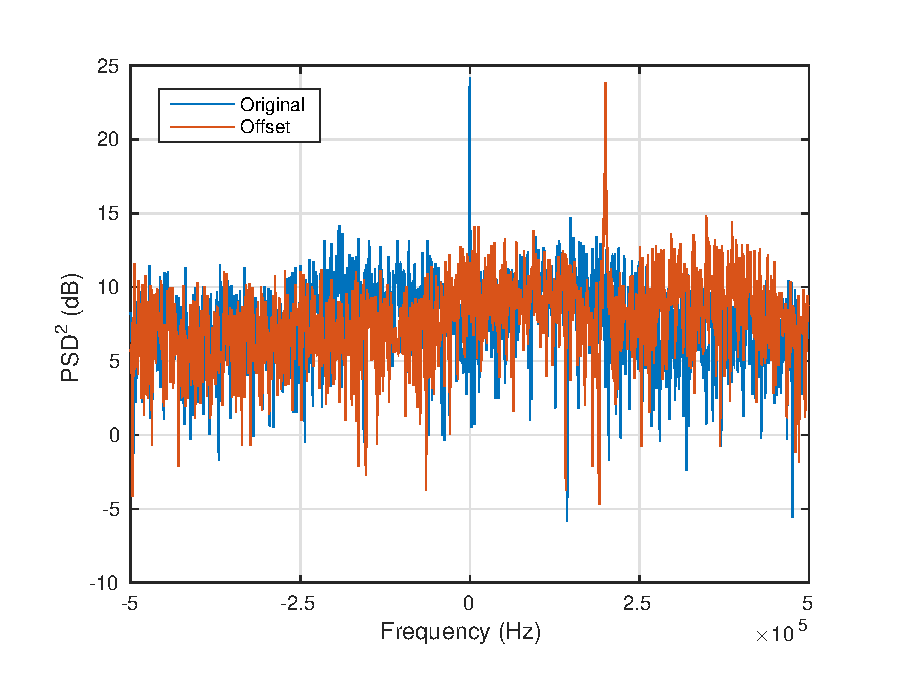
\includegraphics[width=0.8\textwidth]{freqOffsetSquared.eps}
  \caption{PSDs squared of offset and original transmitted signals.}\label{fig:freq_offset_squared}
\end{figure}
%
Alternatively, blind or non-data-aided (NDA) methods can operate over the entire duration of the signal.  
Therefore, it can be argued in a realistic system NDA will outperform DA algorithms.  In this lab we will 
implement a NDA FFT-based technique for coarse compensation.  The concept applied here is straightforward, based on our initial inspection provided in Figure~\ref{fig:freq_offset} we can provide a rough estimate on the symbols offsets.  To make this more accurate for BPSK/DBPSK we can simply square received signal to create Figure~\ref{fig:freq_offset_squared}.  This provides clearly visible peaks at twice the original offset.  The exact algorithm is taken from~\cite{Wang2004}, and $f_o$ can be estimated directly for our BPSK/DBPSK system as follows:
%
\begin{equation}\label{eq:fftcoarse}
 \hat{f}_o = \frac{1}{2\,T\,K} \, \underset{f}{\mathrm{argmax}} \bigl\lvert \sum_{k=0}^{K-1} r^2(k)e^{-j2\pi 
k T/K}\bigr\rvert
\end{equation}
where $K$ is the $FFT$ length.  The estimation in Equation~\eqref{eq:fftcoarse} is defined as coarse since 
the resulting $\hat{f}_o$ can only be one of $K$ values produced by the FFT.  However, we can extend this 
accuracy by interpolating across a fixed set of FFT bins if desired.  The frequency resolution of each FFT bin for the DBPSK system is simply:
%
\begin{equation}
  f_r = \frac{1}{2\,T\,K}.
\end{equation}
Therefore, we can increase the performance of our estimator by increasing the FFT size or decrease the sample 
rate of the signal.

\vbox{
\questionbox{
\begin{enumerate}
 \item Question 0: Based on Equation~\eqref{eq:fftcoarse} implement a coarse frequency correction function in 
MATLAB using the \texttt{fft} function.  Utilize \texttt{lab2part1.m} to help generate the necessary source 
signals.
  \item Question 1: Modify Equation~\eqref{eq:fftcoarse} to handle a Quadrature Phase Shift Keying (QPSK) 
signal instead of DBPSK, and provide a MATLAB function for coarse frequency correction of such a signal.
  \item Question 2: Evaluate the effective range of this FFT method for DBPSK and QPSK.  How would you 
parameterize this estimator for two talking Plutos with these modulation schemes?
  \item Question 3: What are the problems associated with modifying the FFT length and sample rates to change 
the frequency resolution of the estimator?
  \item Question 4: Remove the transmit filters and examine performance over frequency ranges.  Why would 
this change performance?
  \item Question 5: At what angular frequency offset would we still recovery DBPSK without additional 
frequency correction and for how many symbols?
\end{enumerate}
}}

% 
\subsection{Fine Frequency Correction}\label{sec:ffc}
%
After coarse frequency correction (CFO) there will still be offset based upon the configured resolution 
chosen.  Fine frequency correction (FFC), also called carrier phase correction, should produce a stable 
constellation for eventual timing recovery and demodulation.  We describe this correction as producing a 
stable offset, due to how fine frequency offset effects are typically examined with a constellation diagram.  
If a discrete digitally modulated signal exhibits frequency offset, this will cause rotation overtime with a 
constellation diagram.  In Figure~\ref{fig:fine_freq_offset} we demonstrate this effect which was generated 
from the provided script \texttt{lab2part2.m}.  Each number relates a sample's relative occurrence in time, 
and note that if a positive frequency offset is applied the rotation will be counterclockwise and clockwise 
with a negative offset. When the script \texttt{lab2part2.m} is run this effect should be animated by the 
\texttt{comm.ConstellationDiagram} scope.  The rate of the rotation is equal to the frequency offset, which 
is 
another reason it is sometimes defined as $\omega$ (angular frequency).\par
%
\begin{figure}[!htp]
 \centering
  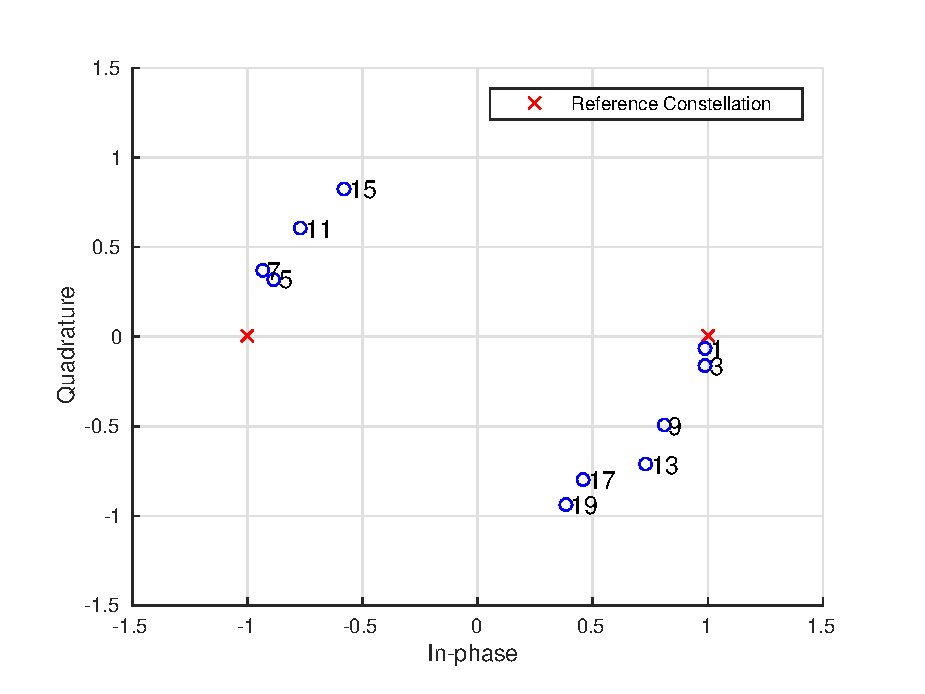
\includegraphics[width=0.8\textwidth]{fineFreqOffset.eps}
  \caption{Constellation of source signal with frequency offset.}\label{fig:fine_freq_offset}
\end{figure}
%
Unlike CFO which uses a feed-forward technique, for FFC we will be using a 
feed-back or closed-loop method based on phase-locked loop (PLL) theory. The structure of this algorithm is 
provided in Figure~\ref{fig:pll_design} derived from~\cite[Chapter~7]{rice2009}, which essentially ``locks'' 
when the error signal $e(k)=\theta-\hat{\theta}(k)$ is driven to zero. This all-digital PLL-based algorithm 
works by first measuring the phase offset of the received sample in the Phase Error Detector (PED), which we 
call the error signal $e(k)$.  The PED is designed based on the structure of the desired receive 
constellation/symbols.  Next, the Loop Filter helps govern the dynamics of the overall PLL.  The Loop Filter 
can determine operational frequency (sometimes called pull-in range), lock time, and dampness/responsiveness 
of the PLL.  Finally, we have the Direct Digital Synthesizer (DDS), whose name is a remnant of analog PLL 
designs with voltage controlled oscillators (VCO).  The DDS is responsible for generation of the correction 
signal for the input, which again will be fed back into the system. In the case of the FFC design, this 
PLL should eventually produce an output signal with desired offset equal to zero.\par
%
When considering our DBPSK system we must design all the components in Figure~\ref{fig:pll_design} 
specifically.  However, we can generalize this design for some modulation schemes.  The instantaneous phase 
error for a rotated DBPSK input signal $y(k)$ can be determined simply by:
%
\begin{equation}\label{eq:e_dbpsk}
 e(k) = sign(Re(y(k))\times Im(y(k))
\end{equation}
%
where $Re()$ and $Im()$ represent the real and imaginary components individually. The reasoning behind 
Equation~\eqref{eq:e_dbpsk} is straightforward to understand.  On the other hand, the Loop Filter in all PLL 
designs is the most challenging aspect, but provides the most control over the adaption of the system.  Here 
we will use a proportional-plus-integrator (PI) filter as our Loop Filter, naming representative of their 
transfer function:
%
\begin{equation}\label{eq:s_xfer}
 F(s) = g_1 + \frac{g_2}{s},
\end{equation}
%
%
\begin{figure}[!htp]
 \centering
 \begin{tikzpicture}[auto, node distance=2cm,>=latex']
    % Blocks and positions
    \node [input, name=input] {};
    \node [block, right of=input, node distance=3cm] (corrector) {Phase Rotator};
    \node [block, below of=corrector, node distance=3cm] (cg) {\begin{tabular}{c} Direct Digital\\Synthesizer  \end{tabular}};
    \node [block, right of=cg, node distance=3.5cm] (lf) {Loop Filter};
    \node [block, right of=lf, node distance=3.5cm] (ed) {\begin{tabular}{c} Phase Error\\Detector \end{tabular}};
    \node [outputMiddle, above of=ed, node distance=3cm] (outputMiddle) {};
    \node [output, right of=outputMiddle, node distance=1cm] (output) {};
    % Lines
    \draw [draw,->] (input) -- node {x(t)} (corrector);
    \draw [-] (corrector) -- node {y(n)} (outputMiddle);
    \draw [->] (outputMiddle) -- node {} (output);
    \draw [->] (outputMiddle) -- node {} (ed);
    \draw [->] (ed) -- node {e(n)} (lf);
    \draw [->] (lf) -- node {f(n)} (cg);
    \draw [->] (cg) -- node {$\phi$(n)} (corrector);
\end{tikzpicture}
  \caption{FFC structure based on PLL design for feed-back corrections.}
  \label{fig:pll_design}
\end{figure}
%
where $g_1$ and $g_2$ are selectable gains. PI filters produce second-order PLLs and only consist of a 
single pole in their transfer function; therefore, they are relatively easy to analyze.  Since we are dealing 
with discrete time signals a z-domain representation is preferable:
%
\begin{equation}\label{eq:z_xfer}
 F(z) = G_1 + \frac{G_2}{1-z^{-1}},
\end{equation}
%
where $G_1\neq g_1$ and $G_2\neq g_2$\footnote{A simple way to translate between Equations~\eqref{eq:s_xfer} 
and~\eqref{eq:z_xfer} is to utilize a bilinear transform.}.  The fractional portion of 
Equation~\eqref{eq:z_xfer}, can be represented nicely by a biquad filter\footnote{See  \texttt{dsp.BiquadFilter}  for a simple realization of a biquad filter.}.\par
%
The last piece to this second-order PLL is the DDS, which is just an integrator.  Since the Filter Loop 
produces a control signal which is equivalent to the frequency of the input signal, it becomes necessary to 
extract the phase of this signal instead.  The transfer functions used for the integrator here are:
%
\begin{equation}
 D(s) = G_3\frac{1}{s} \quad\rightarrow\quad D(z) = G_3\frac{z^{-1}}{1-z^{-1}}.
\end{equation}
%
Note that we have added an additional delay of a single sample in the discrete domain, and since we are 
producing a correction signal $G_3=-1$. Again this integrator can be implemented with a biquad filter.\par
%
In this arrangement of the PLL, filling in the desired responses in Figure~\ref{fig:pll_design}, this system 
should produce an output $y(k)$ which has minimal phase and frequency offsets.  Going around the loop again 
in Figure~\ref{fig:pll_design}, the PED will first produce an error equal to the phase offset associated with 
the observed corrected\footnote{We define this as a corrected symbol since it has passed through the rotator 
and we will not apply addition phase shifts to this sample.  This is also the output of the PLL.} symbol 
$y(k)$, then the Loop Filter will relate this observed error and weight it against all previous errors.  
Finally, the DDS will convert the weighted error/control signal $f(k)$ to a phase $d(k)$ which we use to 
correct the next input sample $x(k+1)$.  In the case of frequency offsets, $d$ will continuously change since 
is it a phase value not a frequency value. However, if the input signal is too dynamic or the gains of the 
filters are not designed appropriately, the PLL will not be able to keep up with the changing phase 
(frequency) of $x$.\par
%
For the calculation of the gain values ($G_1,G_2$) utilize the following equations based on a preferred 
damping factor $\zeta$ and loop bandwidth $B_{Loop}$:
%
\begin{equation}
  \theta = \frac{B_{Loop}}{M(\zeta + 0.25/\zeta)} \quad \quad \Delta = 1 + 2\zeta\theta + \theta^2
\end{equation}
\begin{equation}
  G_1 = \frac{4\zeta\theta/\Delta}{M} \quad \quad G_2 = \frac{(4/M)\theta^2/\Delta}{M}
\end{equation}
%
where $M$ is the constellation order.  Note that $B_{Loop}$ is a normalized frequency.  If you are interested 
in how these are derived, see~\cite[Appendix~C]{rice2009}.  For the selection of $\zeta$:
%
\begin{equation}
 \zeta = \begin{cases}
         \le 1, \text{Underdamp}\\
         =1, \text{Damped}\\
         \ge 1, \text{Overdamped},\\
         \end{cases}
\end{equation}
which will determine the responsiveness and stability of the PLL.  The selection of $B_{Loop}$ should be 
related to the maximum estimated frequency locking range $\Delta_{f,lock}$ range desired:
%
\begin{equation}\label{eq:pullin}
\Delta_{f,pull} = \frac{4(2\pi\sqrt{2}\zeta B_{Loop})^2}{B_{Loop}^3}.
\end{equation}
%
Note that this value is an estimate based off a linearized model of the PLL; therefore inconsistencies may 
exists in the simulated versions. However, this PLL design should perform well even under strong noise 
conditions when configured correctly.  Unlike the CFO correction this FFC will generally not have the same 
operational range.  In your designs is may be useful to start with a damping factor of $\zeta = 
\frac{1}{sqrt{2}}$ and a loop bandwidth of $B_{Loop} = 0.01$.\par
%
With this FFC implementation we can implement a system that provides a stable constellation with minimal 
rotation or frequency offset.  Figure~\ref{fig:fine_freq_offset_constell} provides an initial constellation 
and the resulting constellation after FFC, and Figure~\ref{fig:fine_freq_offset_est} provides an example of 
a converging PLL over time. When determining performance of the FFC there are several common 
methods.  First is to evaluate the mean squared error (MSE) of the estimated offset, and second is to take an 
error vector magnitude (EVM) measurement compared to a reference constellation. EVM measurements can be 
useful because they provide information on the correctness of the signal orientation, which will provide 
insight into possible downstream errors. To calculate EVM in percent RMS use the following equation:
%
\begin{equation}
  EVM_{RMS} = 100\times\sqrt{\frac{\frac{1}{N}\sum_{k=0}^{N-1} e_{const}(k) }{\frac{1}{N}\sum_{k=0}^{N-1} 
(Re(y(k))^2 + Im(y(k))^2) }},
\end{equation}
%
where
\begin{equation}
 e_{const}(k) = (Re(y(k)) - Re(\bar{y}(k)))^2 + (Im(y(k)) - Im(\bar{y}(k)))^2
\end{equation}
and $\bar{y}(k)$ is the reference symbol for $y(k)$.  EVM is a measure on the dispersiveness of the received signal.  Therefore, the lower the EVM values the better.


%
\begin{figure}[!htp]
 \centering
  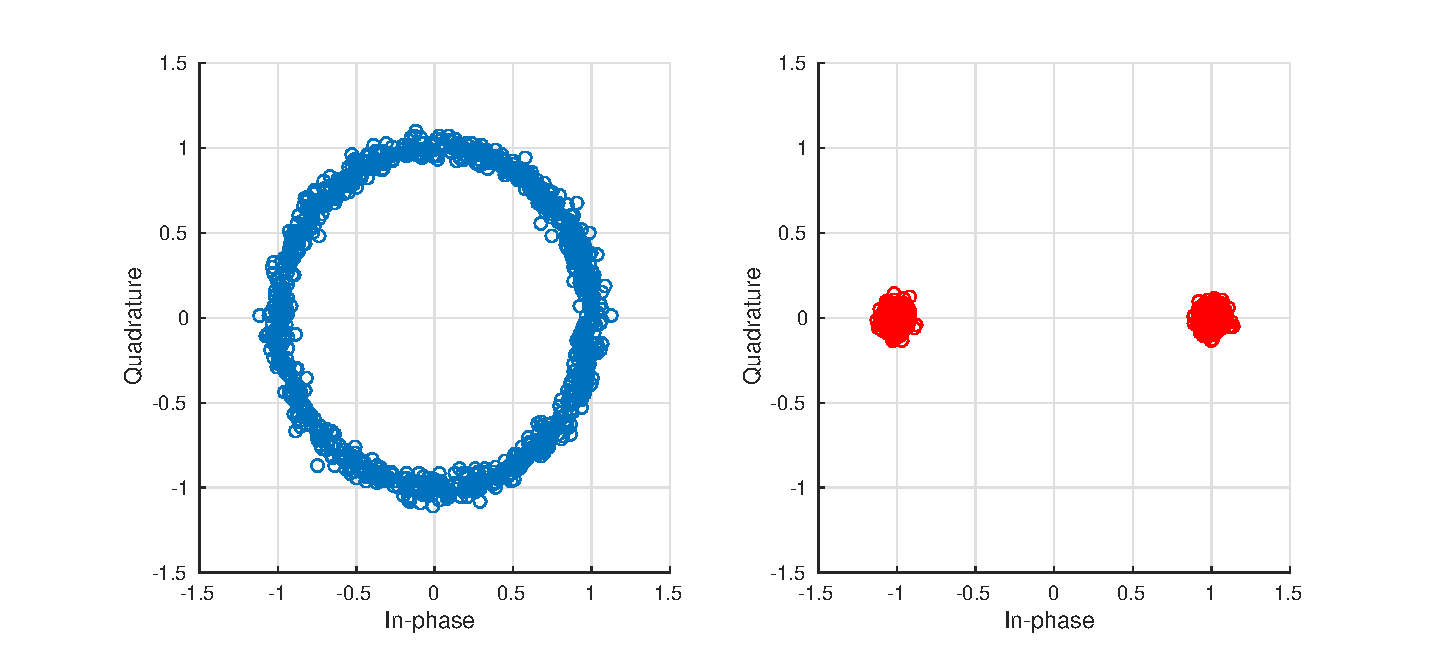
\includegraphics[width=0.9\textwidth]{fixed_correction.eps}
  \caption{Constellation of source signal with frequency offset (left) and corrected 
constellation using FFC PLL design (right).}\label{fig:fine_freq_offset_constell}
\end{figure}
%
\begin{figure}[!htp]
 \centering
  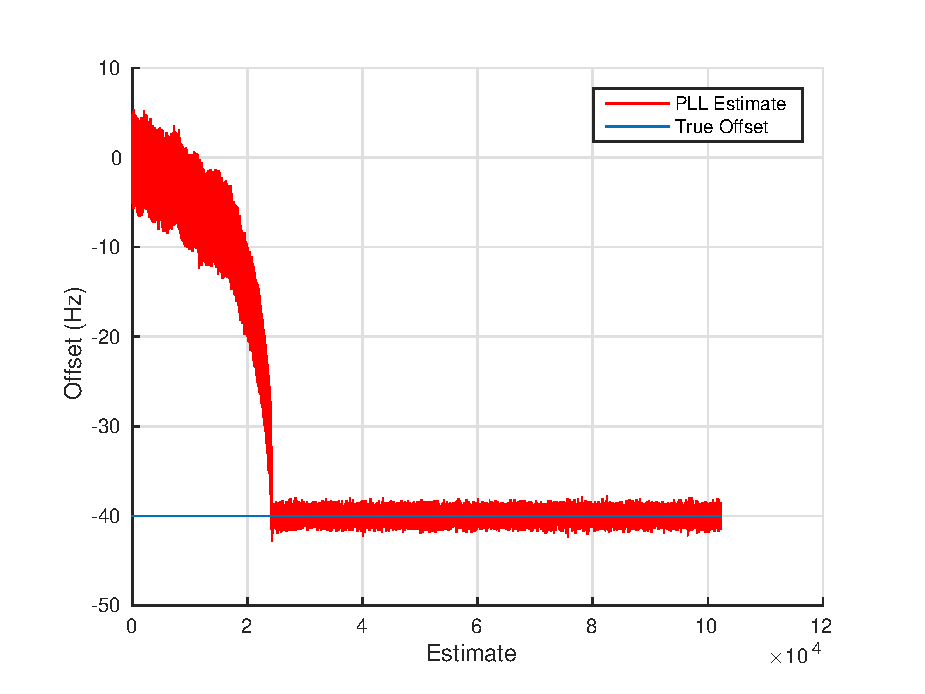
\includegraphics[width=0.8\textwidth]{pll_performance.eps}
  \caption{Estimations over time and converge of implemented PLL.}\label{fig:fine_freq_offset_est}
\end{figure}
%

\vbox{
\questionbox{
\begin{enumerate}
 \item Based on Section~\ref{sec:ffc} implement a FFC in MATLAB. Utilize \texttt{lab2part1.m} to help 
generate the necessary source signals with frequency offsets.
 \item With your constructed FFC, evaluate the effect on convergence times for significant offsets with 
different damping factors and loop bandwidths.  Illustrate scenarios of interest with plots.
 \item From the output of the integrator in your FFC, generate frequency estimates and check them against 
your chosen offset with MSE and EVM evaluations.
 \item With your constructed FFC, evaluate the accuracy of equation~\eqref{eq:pullin} (Do not perform an 
analytical evaluation).
 \item Ignoring timing correction what is the maximum frequency offset DBPSK can handle?  Describe how you 
determined this conceptually.
 \item What would be an appropriate PED for QPSK?
 \item For coherent modulation schemes what additional correction would need to be applied with respect to 
frequency offset?
 \item Evaluate EVM as a function of SNR (in dB) for offsets of $0.1F_s, 0.3F_s$ and $0.5F_s$.
\end{enumerate}
}}

\newpage
\section{Open-ended Design Problem: Automatic Frequency Offset Compensator}

%NEW SYSTEM DIAGRAM WITH SYNCHRONIZERS
%
%COMBINE COARSE AND FINE FREQUENCY CORRECTION IS APPROPRIATE FASHION AND DESCRIBE REASONING

\subsection{Introduction}
Beginning from this laboratory, you will be given an open-ended
design problem at the end of each experiment. These problems are
related to what you have learned and done in each laboratory, but
requires additional thinking and investigation. There is no single
solution for these problems, and each student group is expected to
come up with their own innovative design.

\subsection{Objective}
The objective of this problem is to design and implement a
software-defined radio (SDR) communication system capable of
automatically calculating and correcting the frequency offset between two Pluto
SDRs.

In Sections~\ref{sec:cfo} and~\ref{sec:ffc} you have implemented and simulated carrier frequency correction.  
Now we will introduce the Pluto to replace the channel in Figure~\ref{fig:simple_sys}. In this work you will 
experience real phase and frequency mismatches between transmitters and receivers.  Utilize your previously 
constructed code here to compensate for these new realistic problems.  It will be up to you to configure the 
system, and provide reasoning for this configuration.  We have presented two methods for frequency correction, 
but you are free to use these in any arrangement you want, or use your own algorithms.  However, you must 
provide an evaluation of the overall system performance.  Your final implementation should be tuned to handle 
any set of Pluto radios, not just the ones used by your team.\par
%
With your built frequency correction code perform the following tasks:
%
\begin{enumerate}
 \item First, using a single Pluto transmit your DBPSK reference signal across to the same radio.  It may be 
useful to start with the \texttt{loopback.m} example provided in Lab 0.  Repeat this experiment by increasing 
the center frequency of the transmit or receive chain.  Graph the resulting estimates.
  \item Second, using a pair of Plutos repeat this estimation again as previously performed with a single 
Pluto.  Provide EVM measurements at different distances and/or different gain setting for the radio.
  \item Compare your results here from what you have obtained in Sections~\ref{sec:cfo} and~\ref{sec:ffc}. 
Use statistics to evaluate frequency estimations in your comparisons.
\end{enumerate}
%

% \subsection{Theoretical Background}
% \begin{enumerate}
% \item Before you apply your method to USRP2 boards, it is highly recommended that you test your method with Simulink-only model without USRP and see whether it works.
% \item In the Simulink-only model, you can introduce the frequency offset by \texttt{Phase/Frequency Offset} block. Specify a frequency offset in this block, and see whether
% your Simulink model can give you the number you have specified.
% \item An important hint: If you take the square of a signal, the FFT of the received signal will be shifted double of the frequency offset.
% \item In your model, you might need the following blocks:
% \begin{enumerate}
% \item \texttt{Random Integer Generator}
% \item \texttt{Baseband Modulator}
% \item \texttt{Raised Cosine Transmit Filter}
% \item \texttt{Magnitude FFT}
% \item \texttt{Probe}
% \item \texttt{Maximum}
% \end{enumerate}
% The first three blocks are used on the transmitter side, and the
% last three blocks are used on the receiver side. Using
% \texttt{Probe} and \texttt{Maximum}, you will be able to find the
% location of the peak of the FFT. But of course, you are not
% constrained to these blocks. You can use all the blocks available in
% Simulink. If you want, you can even use MATLAB to implement your
% method.
% \item Although you are required to find the frequency offset of two USRP2 boards, you are actually trying to find the frequency offset of the received signal.
% \item Compare your result here from what you have obtained in Section~\ref{sec:offset}.
% \end{enumerate}
%
% \newpage

\section{Lab Report Preparation \& Submission Instructions}
Include all your answers, results, and source code in a laboratory
report formatted as follows:
\begin{itemize}
 \item Cover page: includes course number, laboratory title, names and student numbers of team, submission
 date.
 \item Table of contents, list of tables, list of figures.
 \item Commentary on designed implementations, responses to laboratory questions, and explanation of
 observations.
 \item Responses to open-ended design problem.
 \item Source code (as an appendix).
\end{itemize}

Remember to write your laboratory report in a narrative approach, explaining your experience and observations in such a way that it provides the reader with some insight as to what you have accomplished.  Furthermore, please include images and outputs wherever possible in your laboratory report document.\\

\noindent Each group is required to submit a single report
electronically (in PDF format) to \texttt{alexw@wpi.edu} by the scheduled due date and time.
Reports that do not meet these specifications will be returned
without evaluation and will receive a grade of ``0'' for the report
segment of the laboratory experiment.


\newpage
\bibliographystyle{plain}
\bibliography{lab1bib}


\end{document}
